\documentclass[12pt, a4paper]{article}
\usepackage[portuguese]{babel}
\usepackage[margin=1in]{geometry}
\usepackage[colorlinks,allcolors=blue]{hyperref}
\usepackage[utf8]{inputenc}
\usepackage{graphicx}
\usepackage{amsmath}

\newcommand{\dpar}[1]{\left(#1\right)}
\newcommand{\un}[1]{\mathrm{#1}}

\DeclareMathOperator{\sen}{sen}

\title{Movimento retilíneo}

\author{Max Jáuregui}
\begin{document}
\maketitle

\section{Velocidades média e instantânea}

Vamos estudar o movimento de um corpo em uma linha reta, a qual vamos considerar como sendo paralela ao eixo $x$.

Se em dois instantes de tempo $t_1$ e $t_2$ o corpo se encontra respectivamente nas posições $x_1$ e $x_2$, definimos o \textbf{deslocamento} do corpo no intervalo $[t_1,t_2]$ por $\Delta x=x_2-x_1$. Definimos também a \textbf{velocidade média} do corpo no intervalo $[t_1,t_2]$ por
$$v_m=\frac{\Delta x}{\Delta t}=\frac{x_2-x_1}{t_2-t_1}\,.$$

Suponhamos que a posição de um automóvel em cada instante de tempo $t$ seja dada por $x(t)=(10\,\un{m}/\un{s}^2)t^2+5\,\un m$. A velocidade média no intervalo $[0\,\un s,1\,\un s]$ é dada por
$$v_m=\frac{x(1\,\un s)-x(0\,\un s)}{1\,\un s-0\,\un s}=\frac{15\,\un m-5\,\un m}{1\,\un s}=10\,\frac{\un m}{\un s}\,.$$
No intervalo $[0,9\,\un s, 1\,\un s]$, a velocidade média será
$$v_m=\frac{x(1\,\un s)-x(0,9\,\un s)}{1\,\un s-0,9\,\un s}=\frac{15\,\un m-13,1\,\un m}{0,1\,\un s}=19\,\frac{\un m}{\un s}\,.$$
Calculando a velocidade média nos intervalos $[0,99\,\un s,1\,\un s]$, $[0,999\,\un s,1\,\un s]$, $\ldots$, vamos perceber que os valores obtidos vão se aproximar cada vez mais de $20\,\un m/\un s$. Logo, é razoável definirmos a velocidade no instante $t=1s$ como sendo $20\,\un m/\un s$. Essa velocidade é chamada de \textbf{velocidade instantânea} e é definida para qualquer instante $t$ por
$$v(t)=\lim_{\Delta t\to 0}\frac{x(t+\Delta t)-x(t)}{\Delta t}\,.$$
O limite do lado direito é conhecido como a \textbf{derivada} de $x(t)$ em relação a $t$ e é denotada por $\frac{dx}{dt}$.

Sobre derivadas precisamos saber o seguinte:
\begin{enumerate}
\item $\frac{d}{dt}[x(t)\pm y(t)]=\frac{dx}{dt}\pm\frac{dy}{dt}$;
\item $\frac{d}{dt}[ax(t)]=a\frac{dx}{dt}$;
\item $\frac{d}{dt}(t^n)=nt^{n-1}$;
\item $\frac{d}{dt}(c)=0$.
\end{enumerate}
Usando essas regras podemos derivar qualquer polinômio; por exemplo, se $p(t)=10t^3-2t^2+6$, então $\frac{dp}{dt}=30t^2-4t$.

Se a posição de um corpo segue a equação $x(t)=(5\,\un m/\un{s}^3)t^3-(10\,\un m/\un{s}^2)t^2+20\,\un m$, qual é a velocidade instantânea do corpo no instante $t=2\,\un s$? A velocidade instantânea em qualquer instante $t$ está dada por
$$v(t)=\frac{dx}{dt}=\dpar{15\,\frac{\un m}{\un{s}^3}}t^2-\dpar{20\,\frac{\un m}{\un{s}^2}}t\,.$$
Logo, no instante $t=2\,\un s$, vamos ter que $v(2\,\un s)=60\,\un m/\un s-40\,\un m/\un s=20\,\un m/\un s$.

\section{Gráficos $x$ versus $t$}
Conhecendo a posição de um corpo, que se move em linha reta, em cada instante de tempo, podemos construir um gráfico $x$ versus $t$ representando os pares ordenados $(t,x(t))$ em um plano cartesiano. O objetivo dessa seção é obter informação sobre o movimento de um corpo a a partit de um gráfico $x$ versus $t$.

Exemplo:
\begin{figure}[ht]
  \centering
  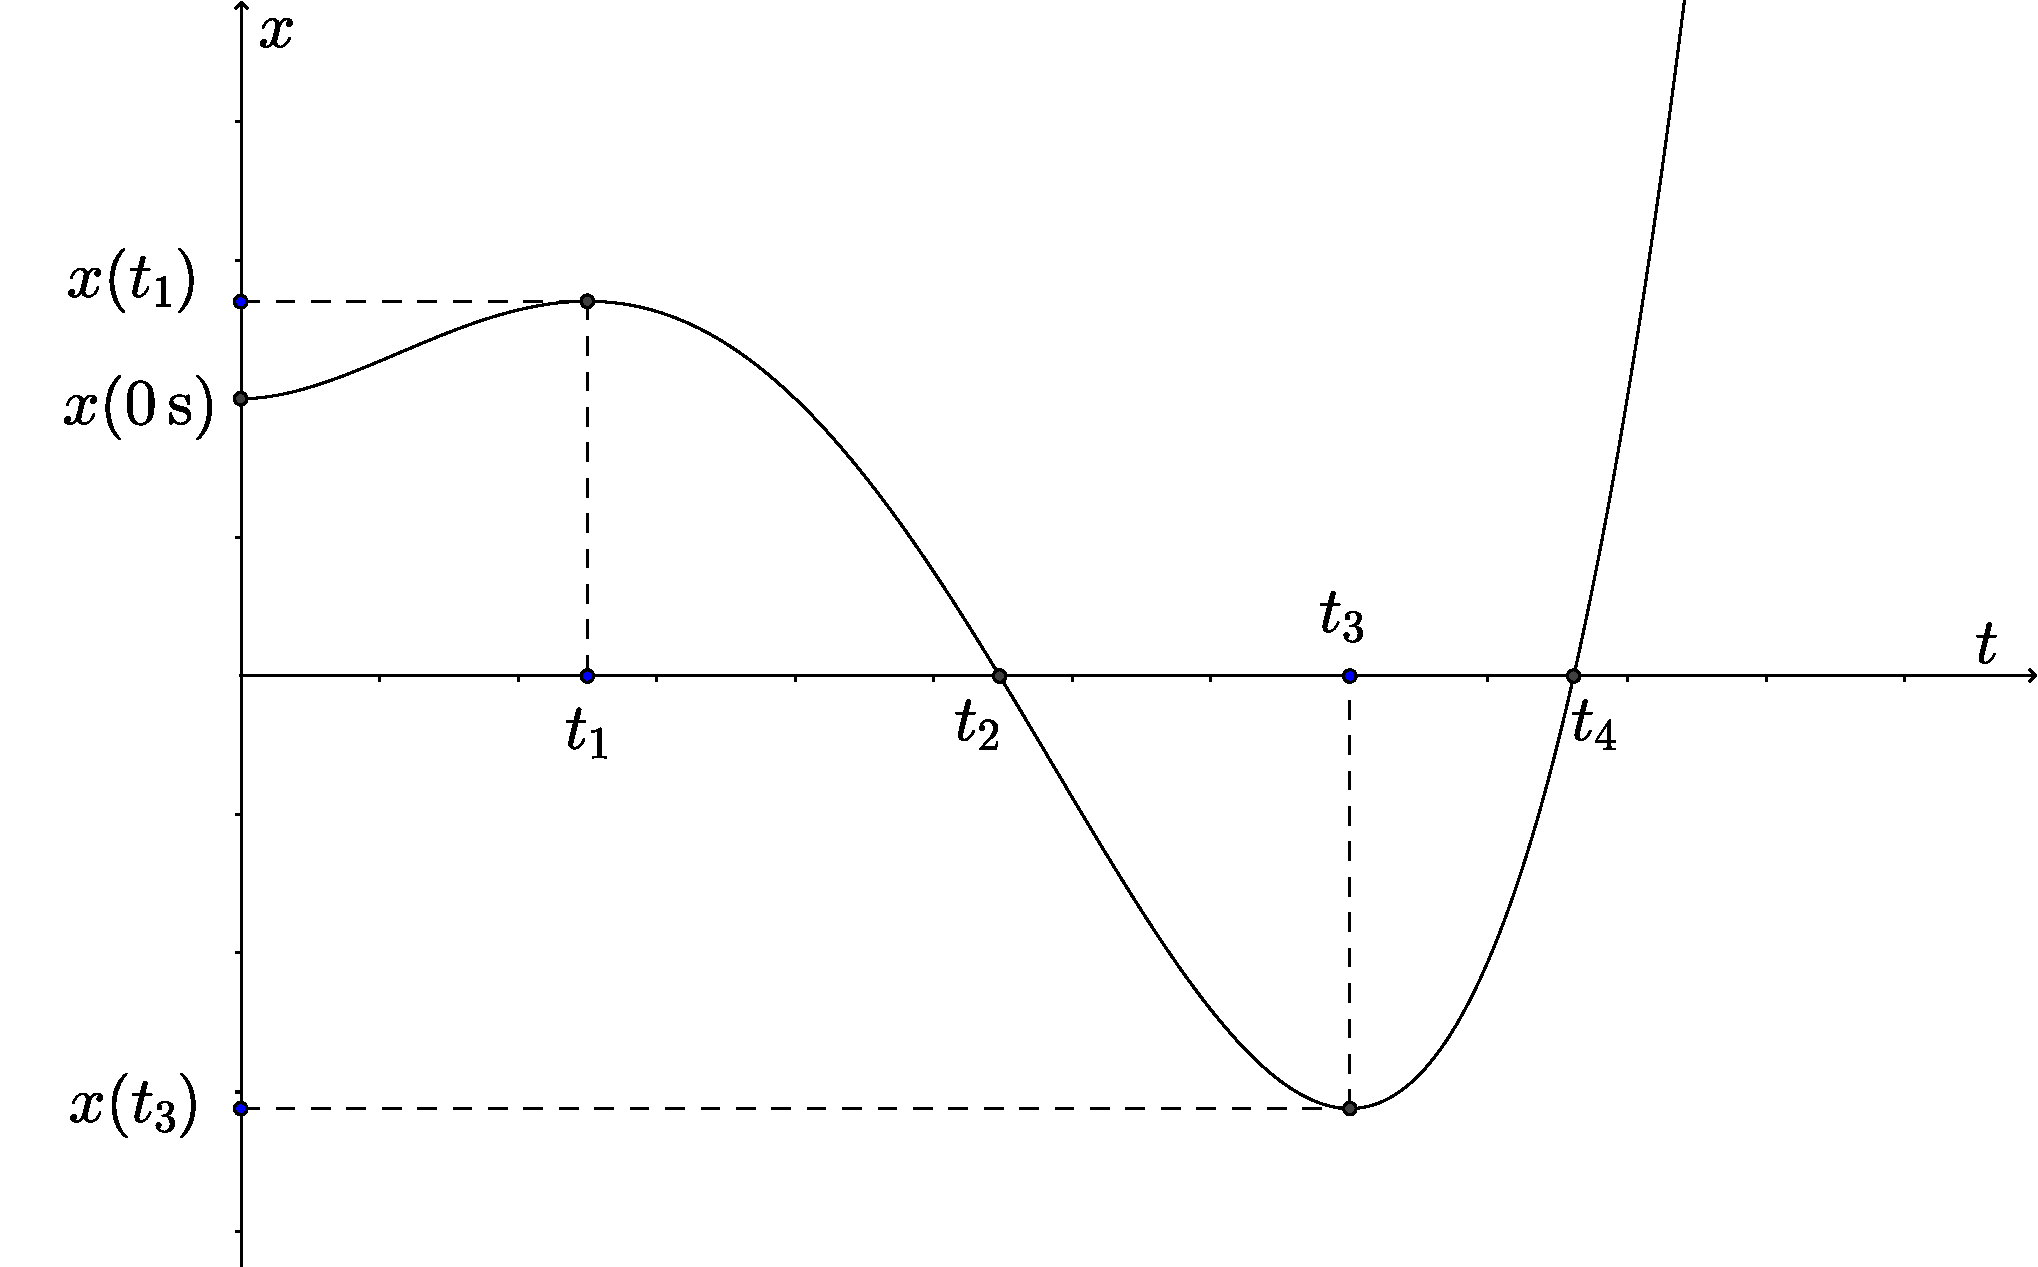
\includegraphics[width=0.9\textwidth,keepaspectratio]{2-movimento-retilineo-fig1.pdf}
  \caption{Exemplo de um gráfico $x$ versus $t$}
  \label{fig1}
\end{figure}
Da figura~\ref{fig1} podemos obter a seguinte informação qualitativa sobre o movimento do corpo: O corpo inicialmente está na origem; logo depois se move à direita (assume valores de $x$ maiores do que $x(0\,\un s)$); no instante $t_1$ o corpo atinge a posição $x(t_1)$ e logo depois desse instante, o corpo se move à esquerda (assume valores de $x$ menores do que $x(t_1)$); no instante $t_2$ o corpo passa pela origem e continua se movendo à esquerda; no instante $t_3$ o corpo atinge a posição $x(t_3)$ e depois desse instante se move à direita passando novamente pela origem no instante $t_4$.

\begin{figure}[ht]
  \centering
  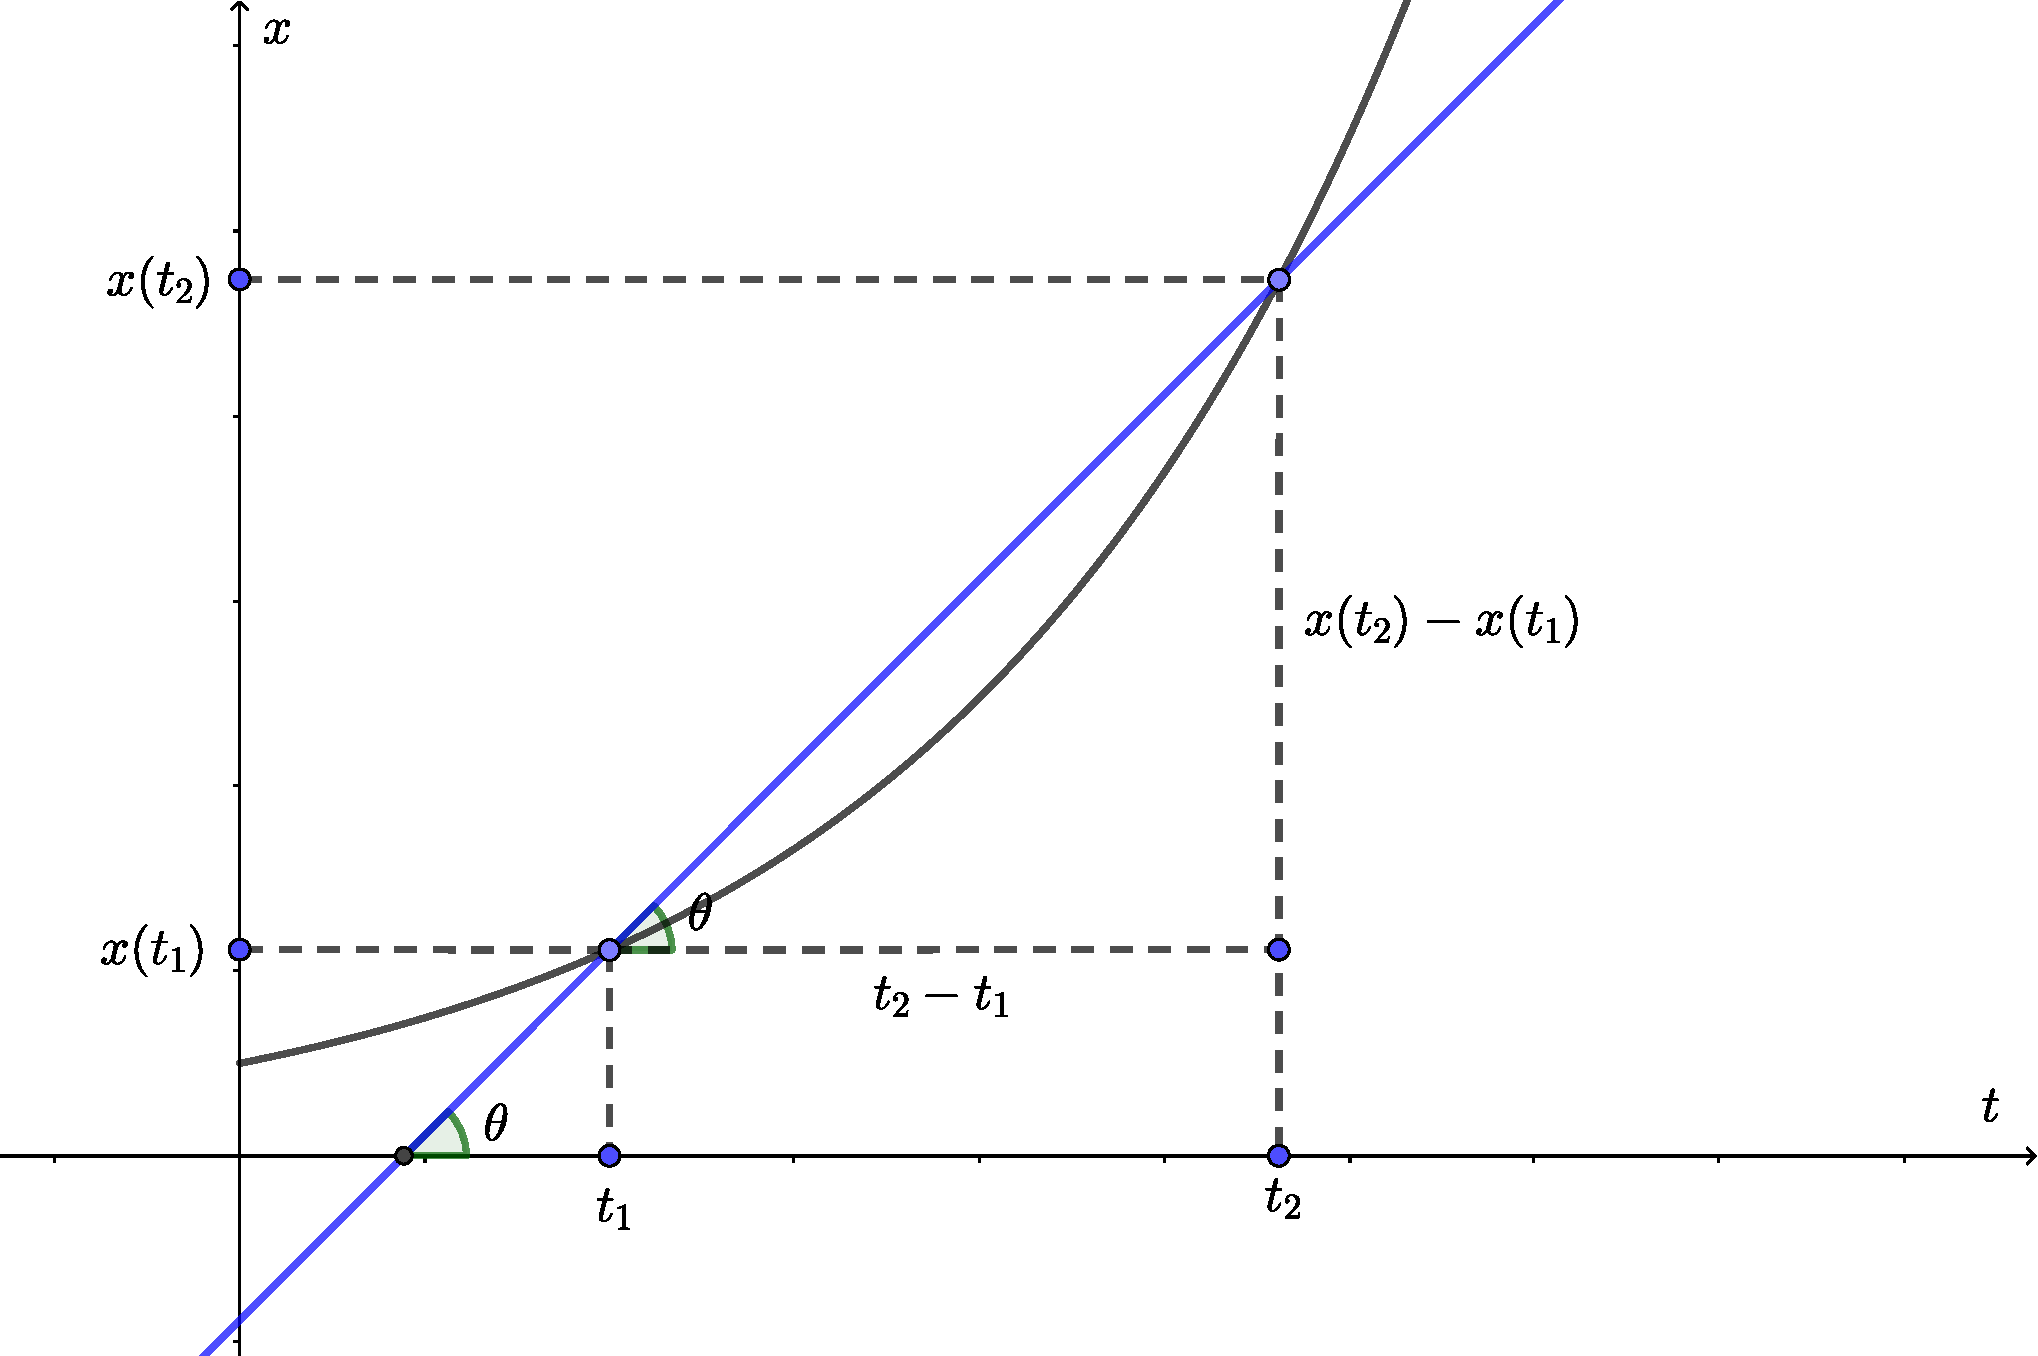
\includegraphics[width=0.9\textwidth,keepaspectratio]{2-movimento-retilineo-fig2.pdf}
  \caption{Cálculo da velocidade média usando um gráfico $x$ versus $t$.}
  \label{fig2}
\end{figure}

\begin{figure}[ht]
  \centering
  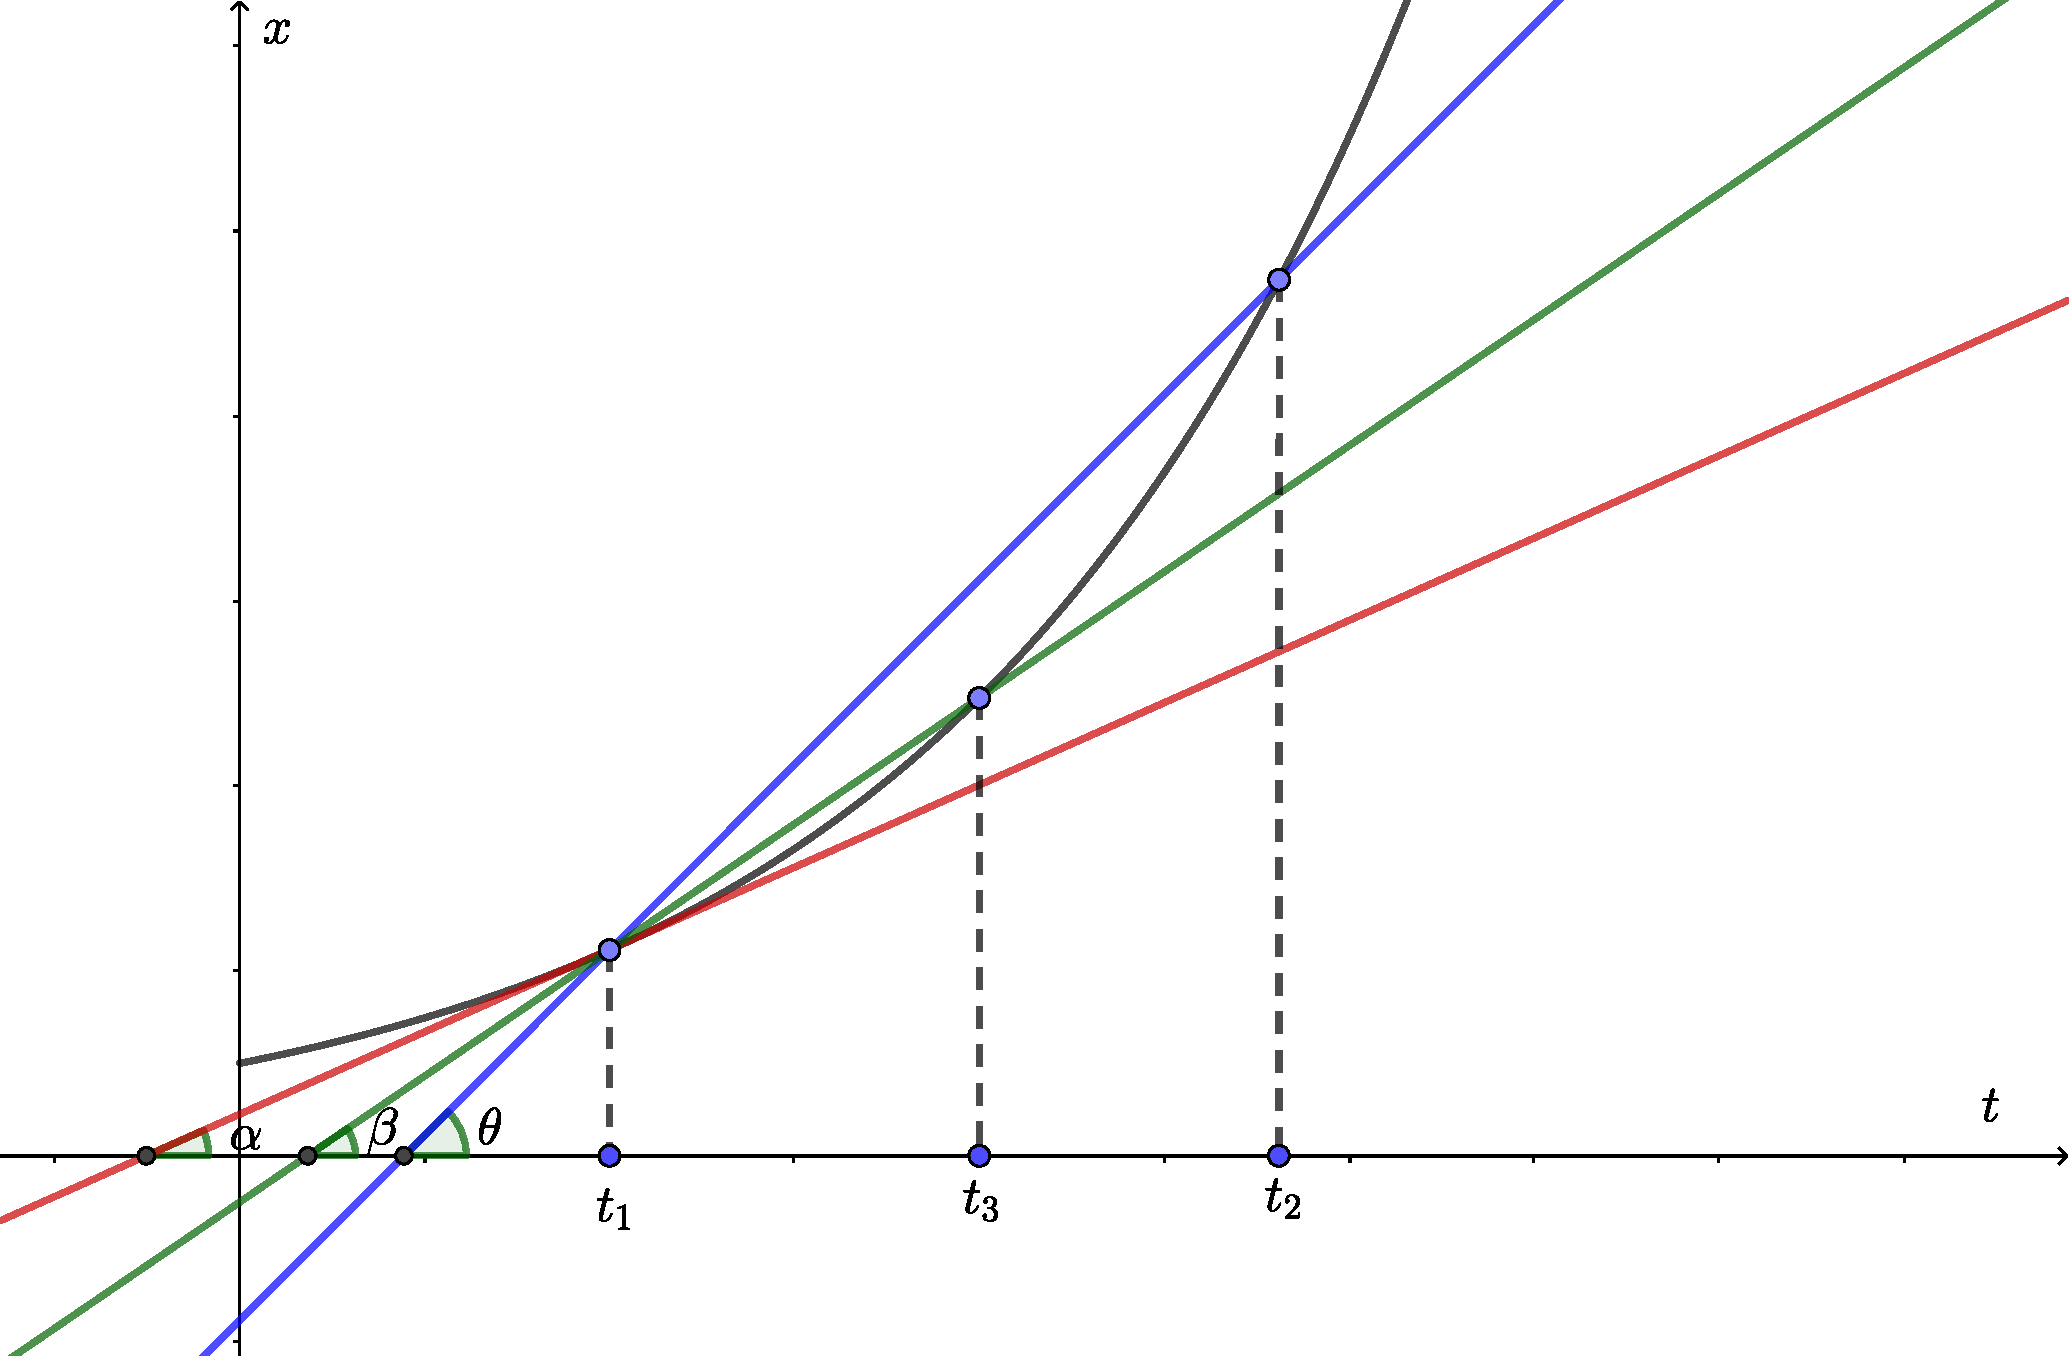
\includegraphics[width=0.9\textwidth,keepaspectratio]{2-movimento-retilineo-fig3.pdf}
  \caption{Cálculo da velocidade instantânea usando um gráfico $x$ versus $t$.}
  \label{fig3}
\end{figure}


Um grafico $x$ versus $t$ também pode nos dar informação sobre as velocidades média e instantânea. Por exemplo, da figura~\ref{fig2} vemos que
$$\tan\theta=\frac{x(t_2)-x(t_1)}{t_2-t_1}\,.$$
Portanto, a velocidade média no intervalo $[t_1,t_2]$ é a tangente do ângulo formado entre o eixo $x$ e a reta secante ao gráfico $x$ versus $t$ que passa pelos pontos $(t_1,x(t_1))$ e $(t_2,x(t_2))$.

Na figura~\ref{fig3} consideramos um instante $t_3$, com $t_1<t_3<t_2$. A velocidade média no intervalo $[t_1,t_3]$ será, pelo que vimos, $\tan\beta$. Considerando instantes $t$ cada vez mais próximos de $t_1$, a reta secante ao gráfico $x$ versus $t$ que passa pelos pontos $(t_1,x(t_1))$ e $(t,x(t))$ vai se aproximar da reta tangente ao gráfico que passa pelo ponto $(t_1,x(t_1))$. Se essa reta tangente faz um ângulo $\alpha$ com o eixo $x$, então $\tan\alpha$ será o valor limite da velocidade média, ou seja, $\tan\alpha$ será a velocidade instantânea no instante $t_1$. Como essa velocidade instantânea é a derivada da função $x(t)$ em relação a $t$ avaliada no instante $t_1$, obtemos a seguinte relação que dá uma interpretação geométrica da derivada:
$$v(t_1)=\frac{dx}{dt}(t_1)=\tan\alpha\,.$$.

\end{document}
